% !Mode:: "TeX:UTF-8"
%!TEX program  = xelatex

%\documentclass{cumcmthesis}
\documentclass[withoutpreface,bwprint]{cumcmthesis} %去掉封面与编号页
\newcommand{\upcite}[1]{\textsuperscript{\textsuperscript{\cite{#1}}}}
\usepackage{subfigure}	%用于排版多张图片
\usepackage{float}	%用于排版图片位置
\usepackage{hyperref}

\usepackage{url}
\title{unsure}

\begin{document}

\maketitle
\begin{abstract}

目前,我国人口形式呈现显著变化,这种变动趋势深刻影响社会发展的各个领域。
本文围绕人口变动及其对高等教育的影响,基于权威数据建立数学模型,
给出了未来20年人口规模的预测值以及人口变化对高等教育水平影响的定量分析,并从人口变动角度量化了学历贬值问题。

针对问题一的人口预测问题,考虑到人口发展的多重影响因素,本文选取了\textbf{经济发展}和\textbf{高等教育发展}两个维度展开分析。
首先,本文采用\textbf{主成分分析法}确定\textbf{GDP}为“经济发展指数”、\textbf{高等教育毛入学率}为“高等教育发展指数”,并采用ARIMA模型对未来20年的这两个指标进行预测。
随后,本文对两个指标进行二次多项式特征拓展,并对历史人口数据进行\textbf{多元非线性回归分析},
得到了未来20年人口规模不断下降的预测趋势,以及不同时期人口规模预测值。
结合预测结果,本文从\textbf{生育支持}、\textbf{女性权益}和\textbf{公共服务}三个方面提出了人口发展政策建议。

针对问题二,本文首先选取了四个核心指标作为\textbf{高等教育发展水平的评价标准}:高等教育生均教育经费、高等学校师生比、高等学校专任教师数占比和研究生毕业生数占比。
考虑到教育指标与时间和人口规模的双重相关性,本文采用\textbf{灰度预测模型}对这四个指标进行未来 20 年的预测,并采用\textbf{归一法}将各指标数值的范围统一到[0,1]。
随后,采用\textbf{熵权法}计算了各个指标的权重,计算逐年各指标得分并合成得到\textbf{逐年教育水平总得分}。
最后,本文通过四个核心指标和高等教育综合得分的动态变化趋势,得出\textbf{结论}:我国高等教育发展水平将在未来20年突破人口规模的限制,保持显著发展态势。

针对问题三,我们探究了\textbf{高学历毕业生的劳动市场供给增速与需求增速的差值($S\_{t}$-$D\_{t}$)},和\textbf{本科以上学历毕业生平均工资比($Y_1$)}及\textbf{失业率($Y_2$)}的关系。
本文以\textbf{归一化}后的年份数据为自变量,以毕业生人数、第三产业占GDP比重、$Y_1$或$Y_2$为因变量作两张\textbf{趋势图},
得出结论:近年来$Y_1$和$Y_2$的不利变化趋势,与$S\_{t}$显著快于$D\_{t}$的时期吻合。
基于上述观察,本文建立了两个经济模型,定量分析\textbf{供需失衡对学历贬值的影响}。
模型一通过线性回归法,建立了$Y_1$和($S\_{t}$-$D\_{t}$)的关系,结果显示高学历毕业生劳动力供需增速差异的升高,导致其相对工资优势下降。
模型二需要引入第二个自变量,建立$Y_2$和($S\_{t}$-$D\_{t}$)、GDP 增长率之间的关系。
结果显示,高学历毕业生劳动力供需增速差异的升高对失业率有显著正向影响,同时,GDP 增长率的提高对失业率有抑制作用。

最后,本文对所建立的模型进行了灵敏度分析和优缺点评价。


\keywords{\quad \quad    } %空格命令

\end{abstract}

%目录
%\tableofcontents

%新的一页
%\newpage

\section{问题重述}

\subsection{问题背景}

当前,我国人口形势出现了显著变化,出生率持续走低,人口发展呈现老龄化、少子化等趋势性特征。
2023年统计数据显示,我国全年出生人口为902万。而2024年出现小幅回升,新出生人口增至954万。
这种人口变动趋势深刻影响社会发展的各个领域,引发了社会各界对教育、经济和社会可持续发展的广泛关注。

自改革开放以来,我国高等教育事业实现了跨越式发展。1981年《学位条例》\upcite{学位条例}的颁布实施,标志着我国开始确立现代学位制度。
经过四十余年的发展,我国已建成规模成熟的高等教育体系。
然而,在人口结构转型的背景下,高等教育发展正面临新的机遇和挑战。

\subsection{问题重述}

\textbf{问题一}:基于权威数据,构建预测模型,分析未来不同时期的人口规模变化,并提出维持人口永续发展的建议;

\textbf{问题二}:建立量化分析模型,解析人口因素对高等教育发展的影响;

\textbf{问题三}:建立量化分析模型,解析人口变动的背景下学历价值稀释的问题。


\section{问题分析}

\subsection{问题一}

问题一要求我们构建科学的数学模型,预测我国未来不同时期的人口规模变化,并提出促进人口长期健康发展的政策建议。
首先,在指标选取方面,基于人口发展的多维度影响因素,我们重点考察经济发展和高等教育发展两个重要维度。
为了更准确地刻画这两个维度的影响,需要采用主成分分析法进行降维处理,分别得到一个“经济发展指数”和“高等教育发展指数”。

在建模方法上,需要采用分步预测的方式。首先基于统计年鉴中的历史数据,对经济发展指数和高等教育发展指数进行时间序列分析,获得未来20年的预测值。
随后,运用多元非线性回归的方法,建立人口规模与这两个综合指数之间的关系模型。
最后,将预测得到的经济和教育指数代入模型,便可得到未来20年的人口规模预测值。

\subsection{问题二}

基于上问预测的人口规模数据,问题二要求我们建立量化分析模型,解析人口因素对高等教育发展的影响。
高等教育发展水平涉及多个维度,因此,首先需要确定评价高等教育的核心指标。
结合现有权威数据,我们选取高等教育生均教育经费、高等学校师生比、高等学校专任教师数占比和研究生毕业生数占比四个关键指标,综合反映高等教育的发展水平。

得到各指标的历史数据后,需要预测未来20年各指标的变化趋势。本研究需要采用多变量灰度预测模型,
综合考虑时间和人口因素对各指标的影响。同时,需要对各指标的预测数据进行归一化处理,确保后续计算的公平性与可比性。

各教育指标的权重需要通过熵权法确定,体现各指标对高等教育综合得分的贡献。
计算权重后,需要进一步计算未来各年单个指标的教育得分,并合成得到各年的教育总得分。为便于进行比较分析,还需要将总得分归一化到60-100分区间。
最后,可以通过综合得分的变化趋势,定量分析人口变化对高等教育的影响。

\subsection{问题三}

学历贬值的规律在于学历的客体与主体间供需不平衡\upcite{学历贬值}。
为了深入分析这一问题,我们从收入和就业两个维度对学历贬值进行量化。
从收入角度来看,学历贬值表现为高学历层次的毕业生相对于其他低学历或社会平均工资的相对收入优势下降;
从就业角度来看,则体现为特定学历层次的毕业生失业率上升。

在明确了学历贬值的定义后,我们需要探究人口变化的影响。
从供给端来看,人口结构的变化直接决定了高学历劳动力市场的供给规模;从需求端来看,经济增长和产业结构升级决定了市场对高学历人才的需求。
核心问题在于,高学历劳动力的供给增速($S$)是否超过了需求增速($D$)。如果供给增长快于需求增长,就会导致学历贬值。

因此,从人口规模变化角度分析学历贬值的关键,在于探究\textbf{高学历劳动力供给增速与需求增速的差异($S-D$)},和\textbf{高等教育人才相对工资优势}及\textbf{失业率}的关系。

为了定量分析这一问题,需要搜集多方面的数据,包括本科及以上毕业生的平均工资与社会平均工资的比值以及本科及以上人群的失业率。
人口方面需要关注研究生毕业生人数,用于衡量新增高学历劳动力的供给。此外,经济数据如第三产业占比,能够反映劳动力市场的需求变化。

在分析方法上,可以通过趋势图直观展示学历贬值与人口变化的关系。
同时,可以通过线性回归模型,直观分析供给增速与需求增速的差异对相对收入优势及失业率的影响。


\section{模型假设}

本文提出以下合理假设:

\begin{itemize}
\item 假设回归模型中扰动项服从独立的正态分布;
\item 不考虑大规模人口迁徙、自然灾害等突发性因素对人口和教育指标的影响;
\item 假设高等教育的评价指标间不存在强相关性
\item 不考虑政策干预、技术进步等外界因素对市场机制的影响

\end{itemize}


\section{符号说明}
\begin{center}
\begin{tabular}{cc}
 \toprule[1.5pt]
 \makebox[0.3\textwidth][c]{符号}	&  \makebox[0.4\textwidth][c]{意义} \\
 \midrule[1pt]
 $ X_{ij} $	    	& 第$i$年的第$j$项教育指标数据   \\ 
 $ Z_{ij} $	        & 归一化后第$i$年的第$j$项教育指标数据  \\
 $ max(X{j}) $      & 第$j$项教育指标在20年预测期内的最大值   \\
 $ min(X{j}) $      & 第$j$项教育指标在20年预测期内的最小值  \\
 $ e_j $            & 第$j$项教育指标的信息熵 \\
 $ g_j $            & 第$j$项教育指标的差异系数 \\
 $ w_j $            & 第$j$项教育指标的权重 \\
 $ M_{ij} $         & 第$i$年的第$j$项教育指标的得分 \\
 $ M_j $            & 第$i$年的教育总得分 \\
\bottomrule[1.5pt]
\end{tabular}
\end{center}

\section{模型的建立与求解}

\subsection{问题一模型的建立与求解}

为了预测我国未来20年的人口规模变化,我们考察经济发展和高等教育发展两个维度,并在统计年鉴中获取1995-2023年的相关统计数据。

\subsubsection{基础指标的主成分分析与未来预测}

在本题中,我们首先对经济发展和高等教育发展两个维度的指标进行主成分分析。结果显示,国内生产总值(GDP)在经济维度的载荷量远高于其他经济指标,毛入学率在高等教育维度的载荷量显著其他高等教育指标,最终选择GDP作为“经济发展指数”,选择毛入学率作为“高等教育发展指数”。

整合统计年鉴中GDP和高等教育毛入学率的数据,我们分别对二者进行时间序列分析,采用ARIMA模型对未来20年的这两个指数进行预测。
\begin{table}[H]
    \centering
    \fontsize{10}{12}\selectfont
    \caption{GDP和高等教育毛入学率的预测结果}
    \begin{minipage}{0.48\textwidth}
        \centering
        \begin{tabular}{|c|c|c|}
        \hline
        年份   & GDP(亿元) & 高等教育毛入学率(\%) \\ 
        \hline
        2024 & 1141306    & 58.8         \\ 
        \hline
        2025 & 1185573    & 60.8         \\ 
        \hline
        2026 & 1229840    & 62.8         \\ 
        \hline
        2027 & 1274107    & 64.7         \\ 
        \hline
        2028 & 1318374    & 66.6         \\ 
        \hline
        2029 & 1362641    & 68.6         \\ 
        \hline
        2030 & 1406908    & 70.6         \\ 
        \hline
        2031 & 1451175    & 72.5         \\ 
        \hline
        2032 & 1495442    & 74.5         \\ 
        \hline
        2033 & 1539709    & 76.5         \\ 
        \hline
        2034 & 1583976    & 78.4         \\ 
        \hline
        \end{tabular}
    \end{minipage}%
    \hfill
    \begin{minipage}{0.48\textwidth}
        \centering
        \begin{tabular}{|c|c|c|}
        \hline
        年份   & GDP(亿元) & 高等教育毛入学率(\%) \\ 
        \hline
        2035 & 1628243    & 80.4         \\ 
        \hline
        2036 & 1672510    & 82.4         \\ 
        \hline
        2037 & 1716777    & 84.3         \\ 
        \hline
        2038 & 1761044    & 86.3         \\ 
        \hline
        2039 & 1805311    & 88.2         \\ 
        \hline
        2040 & 1849578    & 90.2         \\ 
        \hline
        2041 & 1893845    & 92.2         \\ 
        \hline
        2042 & 1938112    & 94.2         \\ 
        \hline
        2043 & 1982379    & 96.1         \\ 
        \hline
        2044 & 2015243    & 97.3         \\ 
        \hline
        2045 & 2076458    & 98.6         \\ 
        \hline
        \end{tabular}
    \end{minipage}
\end{table}
\subsubsection{人口规模的未来预测}

选取主要影响人口的两个变量,即GDP(经济发展指数)和高等教育毛入学率(高等教育发展指数),并进行二次多项式特征扩展。
接下来,用拓展后的特征对历史人口数据进行多元非线性回归建模,建立人口预测模型,实现对未来5年、10年、20年的人口规模预测。

如图\ref{quetion1.1}预测结果显示,未来20年我国人口规模将呈现逐渐下降的趋势,预计到2030年人口总数将降至13.962亿人左右,到2035年将降至13.699亿人,到2045年将降至12.937亿人。

\begin{figure}[H]
    \centering
    \caption{人口规模预测与置信区间}
    \includegraphics[width=0.9\textwidth]{p1.png} % 插入图片
	% \vspace{-1.2cm}
	\label{quetion1.1} % 图像标签,用于引用,设置在caption下方
\end{figure}

\subsubsection{模型诊断与进阶分析}
为量化预测不确定性,我们基于t分布的置信区间计算方法,得到了历史与未来人口数据的置信区间,并在时间序列预测曲线上叠加绘制。如图\ref{quetion1.1}所示,置信区间范围随时间扩大,符合外推预测误差累积的规律。

同时,我们计算了历史数据中人口总数实际值与预测值的偏差,并绘制了残差图,以诊断回归模型的拟合效果。
如图\ref{quetion1.2}所示,绝大多数数据点的残差分布在零基准线附近,表明二次多项式回归模型对人口总数的拟合效果较好。
这种随机分布的残差模式验证了模型假设的合理性,说明当前模型已较好地捕捉了GDP和高等教育毛入学率与人口总数之间的非线性关系。

\begin{figure}[H]
    \centering
    \caption{人口规模预测残差图}
    \includegraphics[width=0.9\textwidth]{p2.png} % 插入图片
    % \vspace{-1.2cm}
    \label{quetion1.2} % 图像标签,用于引用,设置在caption下方
\end{figure}

为体现GDP(亿元)、高等教育毛入学率(\%)与人口总数(万人)之间的非线性关系,我们绘制了如图\ref{quetion1.3}所示的三维曲面图。
曲面呈现平滑的非线性趋势,表明GDP和毛入学率对人口总数的联合影响具有复杂性。
此外,图中红色散点为实际观测值,大部分散点紧邻曲面,进一步验证模型有效性。

\begin{figure}[H]
    \centering
    \caption{多元非线性回归模型人口规模预测三维曲面图}
    \includegraphics[width=0.9\textwidth]{p3.png} % 插入图片
    % \vspace{-1.2cm}
    \label{quetion1.3} % 图像标签,用于引用,设置在caption下方
\end{figure}

\subsubsection{政策建议}
为应对人口规模下降的趋势,实现人口长期均衡发展,我们提出以下政策建议:

1、生育支持政策:一方面,可以扩大现有的生育津贴和育儿补贴等直接经济支持\upcite{经济支持}。此外,可考虑实施递进式补贴政策,
即根据生育孩次逐步提高补贴标准,同时对低收入家庭给予额外补助。同时,可实行税收抵免政策,例如按照子女数量调整个人所得税起征点,切实降低家庭生育成本。

2、女性职业权益:首先,企业应优化生育假期制度,完善企业孕期生育津贴、交通津贴等经济补贴制度\upcite{女性职业}。
同时,可推行"弹性返岗"制度,允许女职工分阶段恢复全职工作。针对企业,政府可推行"生育成本社会化分担"机制,均衡分摊产假成本。
在职业发展方面,建议规定企业在员工生育期间保留其岗位职级,并将产假时间从晋升考评年限中扣除,保障女性在生育期间的职业发展权益。

3、公共服务供给:在实践中着力构建普惠性、专业性、共担性和系统性的托育服务。
同时,要建立托育服务人员职业资格认证体系,提高从业人员待遇,从而促进托育服务的发展。
此外,应积极打造"孕-产-育"全程服务链,包括孕期保健、产后康复、早教指导等一体化服务,真正实现儿童优先、家庭为本的社会支持网络,促进生育友好型社会建设\upcite{托育服务}。

\subsection{问题二模型的建立与求解}

为了定量分析人口规模对高等教育发展的影响,本研究构建了一个系统的分析框架,通过灰度预测模型和熵权法相结合的方式,实现了从数据预测到综合评价的全过程建模。

\subsubsection{高等教育发展指标的选取与预测}

首先,我们选取了四个核心指标作为高等教育发展水平的评价标准:高等教育生均教育经费、高等学校师生比、高等学校专任教师数占比和研究生毕业生数占比,
这些指标从资源投入、师资配置、人才培养等维度全面反映了高等教育的发展状况。

考虑到教育指标与时间和人口规模的双重相关性,我们采用灰度预测模型对这四个指标进行未来20年的预测。(补充描述)

随后,对预测结果进行标准化处理,采用最大-最小归一化方法,将各指标的数值范围统一到[0,1]区间,计算公式如下:
\begin{equation}
    Z_{i j}=\frac{X_{i j}-\min \left(X_j\right)}{\max \left(X_j\right)-\min \left(X_j\right)}
\end{equation}
其中$Z_{ij}$为归一化后第$i$年的第$j$项指标数据,$X_{ij}$为原始指标数据,第$j$项指标在20年预测期内的最大值和最小值分别为$\max(X_j)$和$\min(X_j)$。
指标预测与归一化结果见附录\ref{sec:问题二教育指标预测与标准化结果}。

\subsubsection{高等教育水平的量化分析}

为客观反映各指标在高等教育发展中的相对重要性,我们采用熵权法计算各指标的权重。
首先,计算第$j$项指标的信息熵$e_j$,公式如下:
\begin{equation}
    e_j=-\frac{1}{\ln n} \sum_{i=1}^n\left(\frac{Z_{i j}}{\sum_{i=1}^n Z_{i j}} \ln \frac{Z_{i j}}{\sum_{i=1}^n Z_{i j}}\right)
\end{equation}
其中$n$为预测的指标数量($n$=22)。熵值越低,说明该指标的离散度越高,信息量越集中,对高等教育发展贡献越大。

接下来,计算第$j$项指标的权重$w_j$,利用公式:
\begin{equation}
    w_j=\frac{g_j}{\sum_{j=1}^n g_j}
\end{equation}
其中$g_j=1-e_j$为第$j$项指标的差异系数。各指标信息熵、差异系数和权重计算结果如表\ref{question2.1}所示。

\begin{table}[H]
    \fontsize{10}{12}\selectfont
    \centering
    \caption{各教育指标信息熵、差异系数和权重计算结果}
    \begin{tabular}{|c|c|c|c|}
    \hline
    指标          & 信息熵    & 差异系数   & 权重     \\ \hline
    生均教育经费      & 0.9930 & 0.0070 & 0.2566 \\ \hline
    高等学校师生比     & 0.9877 & 0.0123 & 0.4523 \\ \hline
    高等学校专任教师数占比 & 0.9995 & 0.0005 & 0.0181 \\ \hline
    研究生毕业生数占比   & 0.9926 & 0.0074 & 0.2730 \\ \hline
    \end{tabular}
    \label{question2.1}
\end{table}

最后,计算逐年各指标得分$M_{ij}=100 Z_{ij} \cdot w_j $,并合成得到2025-2045逐年总得分$M_i=\sum_{j=1}^4 M_{ij}$,最终结果如图\ref{question2.5}所示。

\subsubsection{人口因素对高等教育发展的影响分析}

首先,通过四个核心指标的动态变化趋势,可以深入揭示人口变化对高等教育系统的多维影响。
数据分析显示,生均教育经费、高等学校师生比、高等学校专任教师数占比和研究生毕业生数占比四项指标,均与人口变化存在显著负相关,如图\ref{question2.0}所示。
人口每下降1\%,生均教育经费因资源集中效应将提升0.61个百分点,师生比将改善0.53个百分点。
当人口总数从2030年的13.96亿下降至2045年的12.94亿时(降幅7.3\%)时,专任教师占比从14.73\%大幅提升至27.94\%,
研究生占比从11.30\%稳步增长至18.24\%,这直接反映了我国高等教育人口规模将持续快速增长,有力推进以人口高质量发展支撑中国式现代化\upcite{高等教育规模发展}。

\begin{figure}[H]
	\caption{核心指标随年份的变化趋势}
	\label{question2.0}
	\subfigure
	{
		\begin{minipage}[b]{.3\linewidth}
			\centering
			\includegraphics[scale=0.32]{p2.1.png}
		\end{minipage}
	} \quad \quad \quad \quad \quad \quad \quad 
	\subfigure
	{
		\begin{minipage}[b]{.3\linewidth}
			\includegraphics[scale=0.32]{p2.2.png}
		\end{minipage}
	}

	\subfigure
	{
		\begin{minipage}[b]{.3\linewidth}
			
			\includegraphics[scale=0.32]{p2.3.png}
		\end{minipage}
	} \quad \quad \quad \quad \quad \quad \quad
	\subfigure
	{
	\begin{minipage}[b]{.3\linewidth}
		\includegraphics[scale=0.32]{p2.4.png}
	\end{minipage}
	}
\end{figure}

其次,总体分析可得,在人口总量持续减少(2024-2045年)与社会经济持续发展的双重作用下,
我国高等教育综合得分呈现明显的上升趋势,如图\ref{question2.2}所示。

两条曲线形成的“剪刀差”图形生动地体现了我国高等教育质量的显著提升,
具体来看,得分曲线的上升过程可以分为三个阶段:2024-2030年是平稳上升期,每年增长幅度较为均匀;2031-2040年进入加速上升期,这段时间的增长斜率相对增大;
2041年后虽然增速有所放缓,但仍保持稳定上升态势。

\begin{figure}[H]
    \centering
    \caption{人口总数和高等教育得分随年份的变化}
    \includegraphics[width=0.9\textwidth]{p2.5.png} % 插入图片
	% \vspace{-1.2cm}
	\label{question2.2} % 图像标签,用于引用,设置在caption下方
\end{figure}

综上所述,我国高等教育发展水平将在未来20年突破人口规模的限制,保持显著发展态势。
这充分展现了高等教育系统在人口转型背景下的强大发展韧性,推进我国在人口新常态下实现教育现代化。
\subsection{问题三模型的建立与求解}

\subsubsection{学历贬值问题中定量分析模型的建立}

在数据处理上,我们搜集了本科及以上毕业生的平均工资与社会平均工资的比值、本科及以上人群的失业率、研究生毕业生人数和第三产业占GDP比重的权威数据,并进行标准化处理。

本研究首先通过趋势图直观展示学历贬值与人口变化的关系。在趋势图中,以因变量毕业生人数($S$)代表高学历劳动力的市场供给,以因变量第三产业占GDP比重($D$)代表市场对高学历人才的需求,二者能够体现人口变化的影响。
左图中,以本科以上毕业生平均工资比($Y_1$)作为因变量,其变化能够反映学历贬值的收入维度。右图中,将$Y_1$替换为$Y_2$,即本科以上学历人群的失业率,从就业维度反映学历贬值。

\begin{figure}[H]
    \centering
    \caption{1992-2023年三个标准化值折线图}
    \includegraphics[width=0.9\textwidth]{p3.1.png} % 插入图片
	% \vspace{-1.2cm}
	\label{question3.1} % 图像标签,用于引用,设置在caption下方
\end{figure}

\begin{figure}[H]
    \centering
    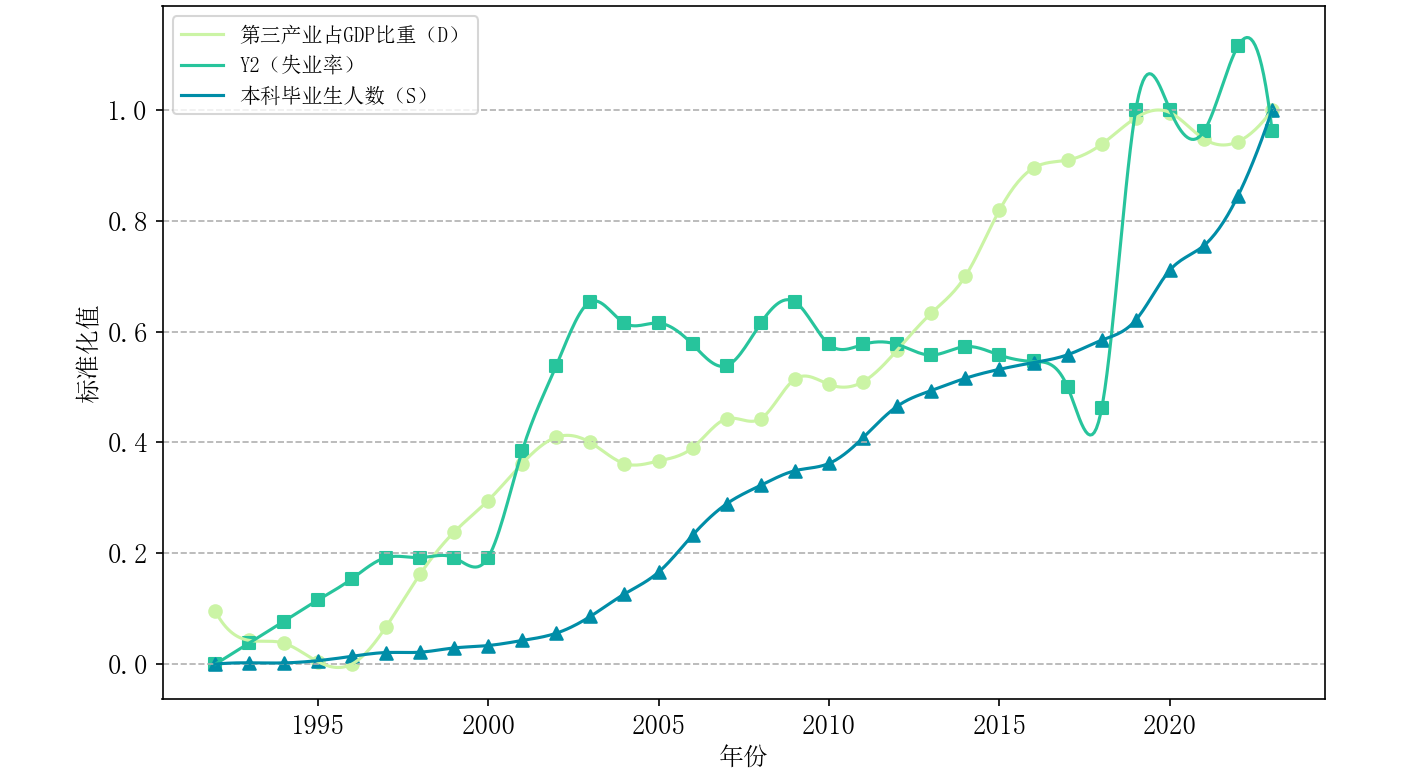
\includegraphics[width=0.95\textwidth]{p3.2.png} % 插入图片
	% \vspace{-1.2cm}
\end{figure}
如图\ref{question3.1}中两张趋势图所示:2017-2023年间,$S$的增长显著快于$D$的增长,与此同时,$Y_1$呈下降趋势,$Y_2$呈上升趋势。
2002-2005年间,当$S$的增长显著快于$D$的增长时,$Y_1$反而呈上升趋势,这是因为二十一世纪初各个行业均在飞速发展,学历贬值现象尚不明显。
综合分析可得,近年来$Y_1$和$Y_2$的不利变化趋势,与$S$增长显著快于$D$增长的时期吻合。

基于上述观察,我们建立了两个经济模型,定量分析供需失衡对学历贬值的影响。

1、模型一:学历贬值在收入维度的表现

模型一通过线性回归法,利用2014-2023年的相关数据,建立高学历毕业生相对工资比和供给速度差之间的关系:
\begin{equation}
    Y_1 \_{t}=\beta_0+\beta_1 \cdot (S\_{t}-D \_{t})+\varepsilon \_{t}
\end{equation}
其中,因变量$Y_1 \_{t}$表示第$t$年的工资比值。$S \_{t}$表示第$t$年本科毕业生人数增长率(\%),代表供给增长速度;$D \_{t}$表示第$t$年第三产业占GDP比重增长率(\%),代表需求增长速度。
核心自变量$S \_{t}-D \_{t}$表示第 t 年高学历劳动力的供给速度超过需求速度的程度。
$\beta_0$为常数项,$\varepsilon \_{t}$为随机误差项。

模型计算结果如图\ref{question3.2}所示。$\beta_1$ < 0且统计显著,证明了高学历毕业生劳动力供需增速差异的升高,导致其相对工资优势下降。
\begin{figure}[H]
    \centering
    \caption{高学历毕业生工资比值与供给增速差的关系}
    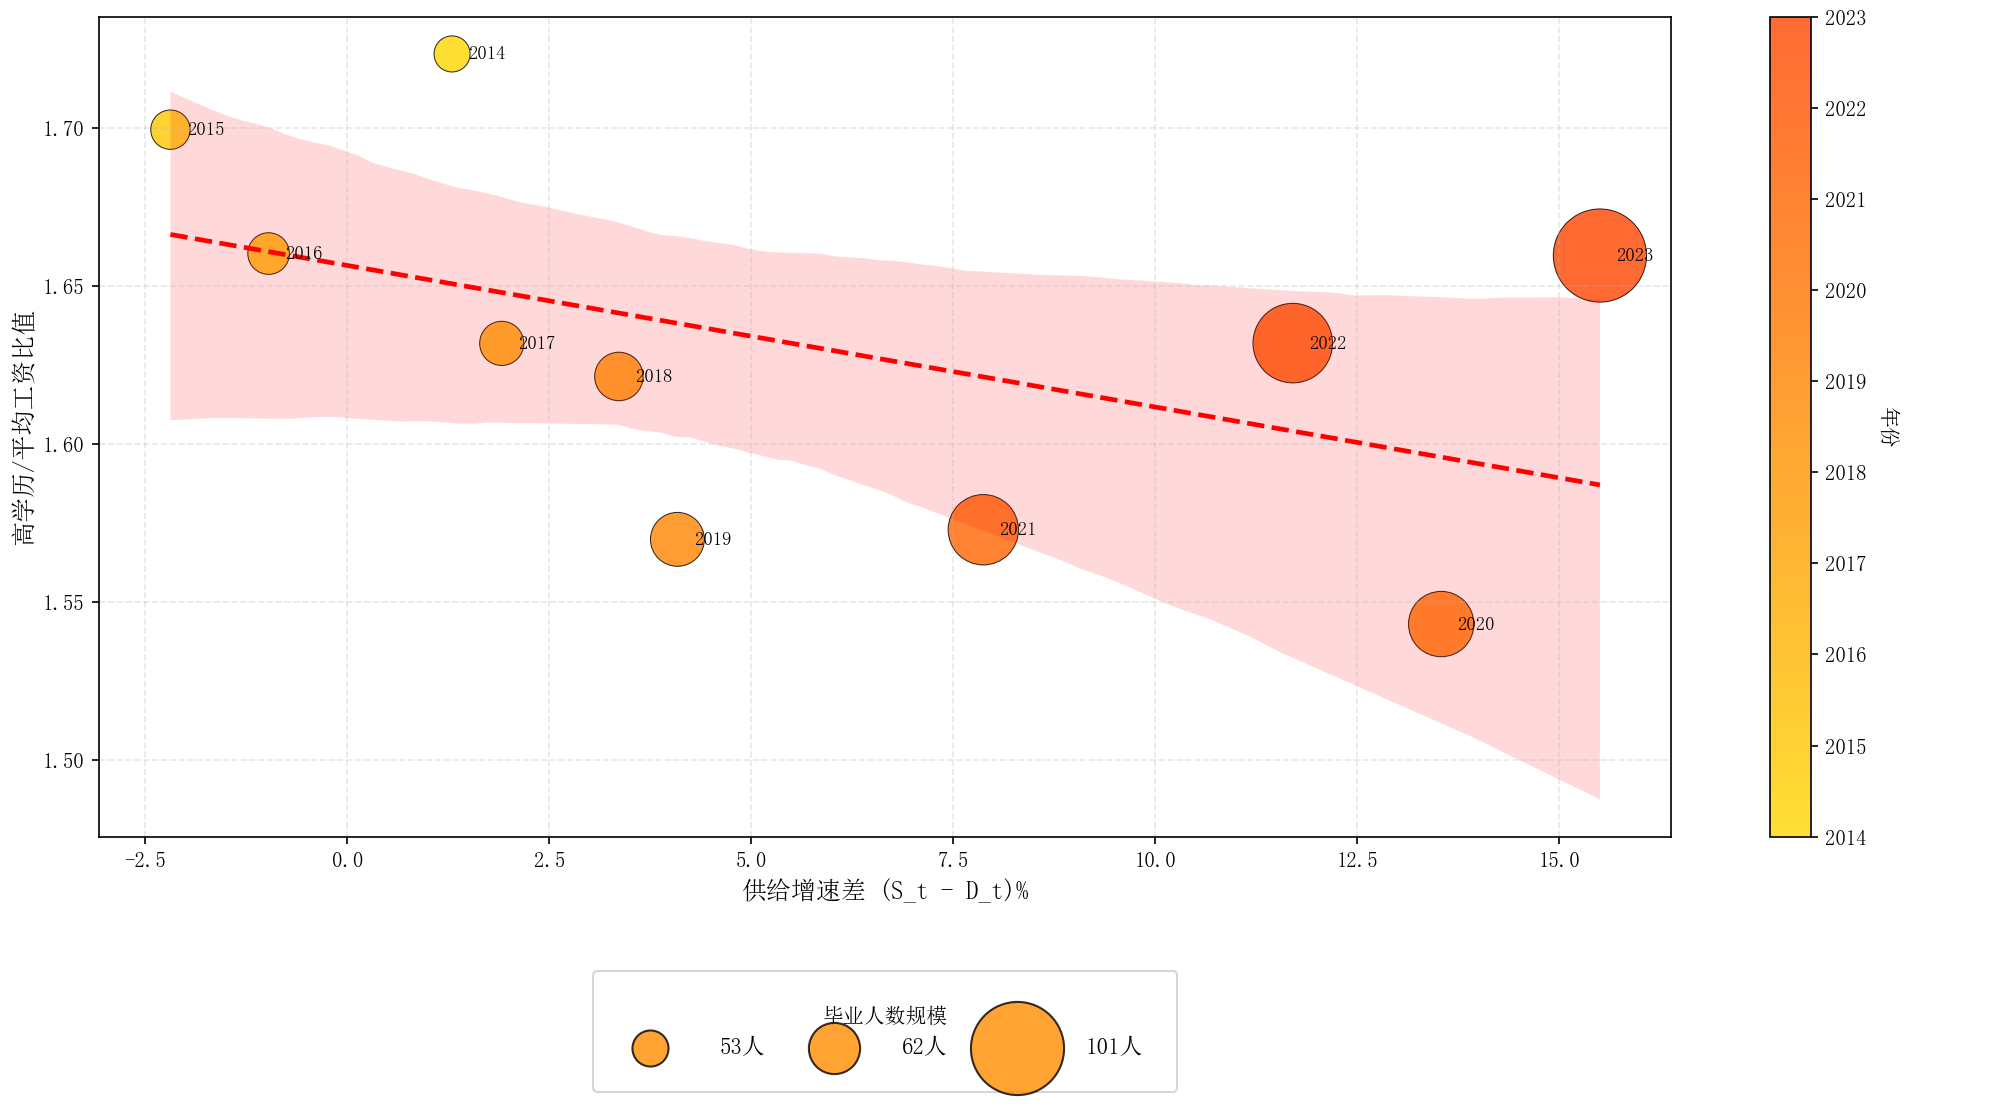
\includegraphics[width=0.95\textwidth]{p3.3.png} % 插入图片
	% \vspace{-1.2cm}
	\label{question3.2} % 图像标签,用于引用,设置在caption下方
\end{figure}

2、模型二:学历贬值在就业维度的表现

由于失业率本身会受到经济周期的影响,故而模型二需要引入第二个自变量,建立高学历毕业生失业率和供给速度差、GDP增长率之间的关系:
\begin{equation}
    Y_2 \_{t}=\beta_0+\beta_1 \cdot (S\_{t}-D \_{t})+\beta_2 \cdot G \_{t}+\varepsilon \_{t}
\end{equation}
其中,因变量$Y_2 \_{t}$表示第$t$年的失业率,新增自变量$G \_{t}$表示GDP增长率。

模型计算结果如图\ref{question3.3}所示。一方面,高学历毕业生劳动力供需增速差异的升高,对失业率有显著正向影响;另一方面,GDP增长率的提高对失业率有抑制作用。
这一结果不仅验证了供需失衡对就业市场的负面影响,同时表明,经济增长本身是降低失业率的关键因素,揭示了经济周期对失业率的调节作用。
\begin{figure}[H]
    \centering
    \caption{供给过剩和经济增长对失业率的影响}
    \includegraphics[width=0.95\textwidth]{p3.4.png} % 插入图片
	% \vspace{-1.2cm}
	\label{question3.3} % 图像标签,用于引用,设置在caption下方
\end{figure}

\begin{figure}[H]
    \centering
    \includegraphics[width=0.95\textwidth]{p3.5.png} % 插入图片
	% \vspace{-1.2cm}
\end{figure}

\subsubsection{人口因素对学历贬值影响的总结分析}

首先,本研究通过系统分析揭示了学历贬值现象的形成机制与表现特征。从供给端来看,80年代末至90年代初的人口出生高峰为后续高等教育扩张提供了基础人口规模。
2003年启动的高校扩招政策使得这批人口在2010-2018年间集中转化为本科毕业生供给。
这种人口结构驱动的供给激增具有典型的周期性特征,其影响在劳动力市场上持续释放,构成了学历贬值的供给端基础。

需求端的分析揭示了深层次的结构性矛盾。虽然我国第三产业占比在2017-2023总体呈现上升趋势,但其增速仍然显著落后于本科毕业生供给增速。
这体现了劳动力市场供需的长期结构性失衡,进而导致学历在劳动力市场的贬值。

学历贬值具有双重表现:从收入维度上看,高学历毕业生劳动力供需增速差异的升高,导致了其相对工资优势下降;
在就业维度,本科毕业生供需失衡是导致其失业率上升的重要因素。
综合分析,人口结构驱动的供给冲击($S$),叠加需求($D$)未能同步跟上,导致了学历在劳动力市场的双重贬值——收入水平下降和就业难度加大。

\section{模型的分析}

\section{模型的评价}

%最后采用的是外面导入bib文件形式
\bibliographystyle{unsrt}
\bibliography{book}

\newpage
%附录
\appendix
\section{源代码}

\newpage

\section{问题二教育指标预测与标准化结果}
\label{sec:问题二教育指标预测与标准化结果}
\begin{table}[H]
    \fontsize{7}{10}\selectfont
    \centering
    \begin{tabular}{|c|c|c|c|c|c|c|c|c|}
    \hline
    年份   & 生均教育经费(元) & 标准化1  & 师生比    & 标准化2  & 高等学校专任教师数占比 & 标准化2  & 研究生毕业生占比 & 标准化1  \\ \hline
    2024 & 158921    & 0.000 & 18.120 & 0.000 & 0.113       & 0.000 & 0.093    & 0.000 \\ \hline
    2025 & 164512    & 0.035 & 18.250 & 0.037 & 0.118       & 0.031 & 0.096    & 0.035 \\ \hline
    2026 & 170293    & 0.071 & 18.390 & 0.076 & 0.123       & 0.063 & 0.099    & 0.070 \\ \hline
    2027 & 176271    & 0.108 & 18.530 & 0.116 & 0.129       & 0.097 & 0.102    & 0.108 \\ \hline
    2028 & 182453    & 0.146 & 18.670 & 0.156 & 0.135       & 0.132 & 0.106    & 0.146 \\ \hline
    2029 & 188847    & 0.186 & 18.820 & 0.198 & 0.141       & 0.169 & 0.109    & 0.186 \\ \hline
    2030 & 195461    & 0.227 & 18.970 & 0.241 & 0.147       & 0.207 & 0.113    & 0.227 \\ \hline
    2031 & 202304    & 0.269 & 19.120 & 0.283 & 0.154       & 0.247 & 0.117    & 0.269 \\ \hline
    2032 & 209384    & 0.313 & 19.280 & 0.329 & 0.161       & 0.289 & 0.121    & 0.314 \\ \hline
    2033 & 216711    & 0.359 & 19.440 & 0.374 & 0.168       & 0.333 & 0.125    & 0.360 \\ \hline
    2034 & 224293    & 0.406 & 19.610 & 0.422 & 0.176       & 0.379 & 0.129    & 0.406 \\ \hline
    2035 & 232140    & 0.455 & 19.780 & 0.470 & 0.184       & 0.427 & 0.134    & 0.455 \\ \hline
    2036 & 240262    & 0.505 & 19.960 & 0.521 & 0.192       & 0.478 & 0.138    & 0.506 \\ \hline
    2037 & 248669    & 0.557 & 20.140 & 0.572 & 0.201       & 0.530 & 0.143    & 0.558 \\ \hline
    2038 & 257371    & 0.611 & 20.330 & 0.626 & 0.210       & 0.585 & 0.148    & 0.611 \\ \hline
    2039 & 266379    & 0.667 & 20.520 & 0.680 & 0.220       & 0.642 & 0.153    & 0.667 \\ \hline
    2040 & 275704    & 0.725 & 20.720 & 0.737 & 0.230       & 0.702 & 0.158    & 0.725 \\ \hline
    2041 & 285357    & 0.785 & 20.920 & 0.793 & 0.240       & 0.765 & 0.163    & 0.785 \\ \hline
    2042 & 295350    & 0.847 & 21.130 & 0.853 & 0.251       & 0.831 & 0.169    & 0.846 \\ \hline
    2043 & 305695    & 0.911 & 21.340 & 0.912 & 0.263       & 0.900 & 0.174    & 0.911 \\ \hline
    2044 & 312769    & 0.955 & 21.490 & 0.955 & 0.271       & 0.948 & 0.178    & 0.954 \\ \hline
    2045 & 320015    & 1.000 & 21.650 & 1.000 & 0.279       & 1.000 & 0.182    & 1.000 \\ \hline
    \end{tabular}
\end{table}

\end{document}